\paragraph{La classe Object}

\begin{minipage}
    {\linewidth}
    \centering
    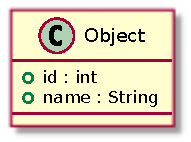
\includegraphics[width=0.80\linewidth]{../schemas/Conception_detaillee/classe_object.pdf}
    \captionof{figure}{Diagramme de classe de Object}
\end{minipage}

\subparagraph{Philosophie de conception \newline} 

\medspace

La classe Object définit les attributs des objets. 

\subparagraph{Description structurelle \newline}

\medspace

\textbf{Attributs :}

\begin{itemize}
    \item \textbf{id : int} --- Identifiant unique et interne à l'application de l'objet afin de l'identifier. 
    \item \textbf{name : String } --- Nom de l'objet. 
\end{itemize}


\textbf{Services offerts :}

N.A.